\documentclass[border=4pt]{standalone}
\usepackage{tikz}
\usetikzlibrary{arrows.meta,shapes.geometric}
\begin{document}
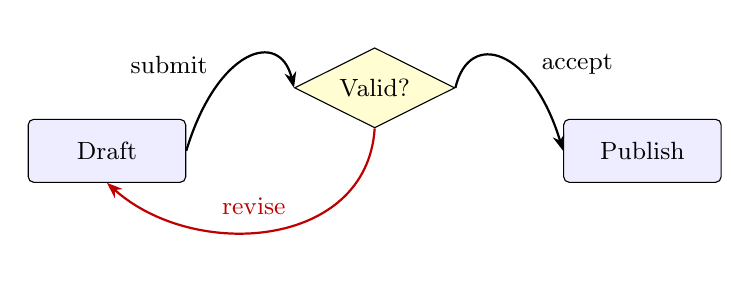
\begin{tikzpicture}[
  auto,
  stage/.style={draw,rounded corners=2pt,minimum width=20mm,minimum height=8mm,fill=blue!7},
  gate/.style={draw,diamond,aspect=2,minimum width=19mm,minimum height=10mm,fill=yellow!18},
  flow/.style={-{Stealth[length=2mm]},thick},
  every node/.append style={font=\small}
]
  \node[stage] (draft) at (0,0) {Draft};
  \node[gate] (review) at (3.4,0.8) {Valid?};
  \node[stage] (ship) at (6.8,0) {Publish};

  \draw[flow] (draft.east) .. controls (1.4,1.3) and (2.2,1.55) .. (review.west)
    node[pos=.28] {submit};
  \draw[flow] (review.east) .. controls (4.6,1.55) and (5.4,1.3) .. (ship.west)
    node[pos=.72] {accept};
  \draw[flow,red!75!black] (review.south) .. controls (3.3,-1.25) and (1.1,-1.4) .. (draft.south)
    node[pos=.42,swap] {revise};
\end{tikzpicture}
\end{document}
